\chapter{Implementation and Performance Analysis}

The core implementation is purposed at the official repository of the MLANN paper by Professor Savchenko. The algorithm is already implemented in \textit{C++} and Caffe by Professor Savchenko and is available via \href{https://github.com/HSE-asavchenko/HSE_FaceRec/tree/master/src}{this} link. I've also provided the \textit{C++} implementation in the directory of this project. In this section, we'll analyze the implementation of MLANN method using Tensorflow and OpenCV in Python.

\section{The Architecture}
Figure 3.1 illustrates the overall architecture of implementation.
\begin{figure}[!h]\centering
	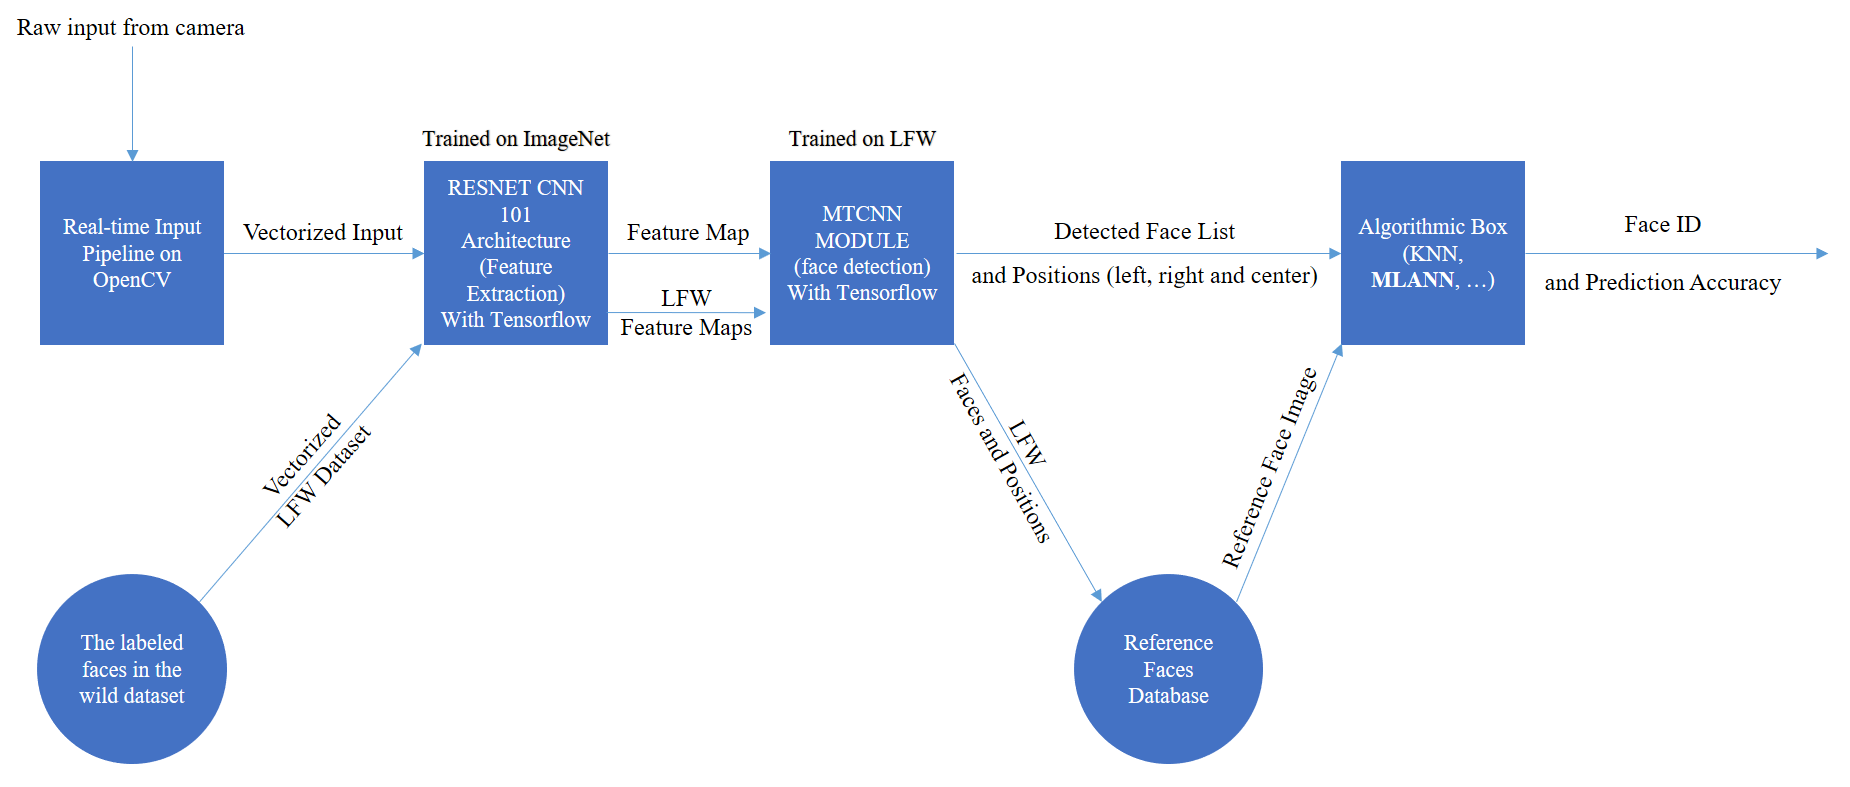
\includegraphics[width=1.1\textwidth]{diagram.PNG}
	\caption{The architecture of real-time face recognition system.}
	\label{pl1}
\end{figure}

\section{Performance Analysis}
Figure 3.2 compares methods of face recognition on LFW dataset. The brute-force method is the worst algorithm possible for face recognition. The proposed method \textit{Pivot based MLANN} has the best performance on this dataset and it is 3.5-5.5 times faster than the brute-force method.
\begin{figure}[!h]\centering
	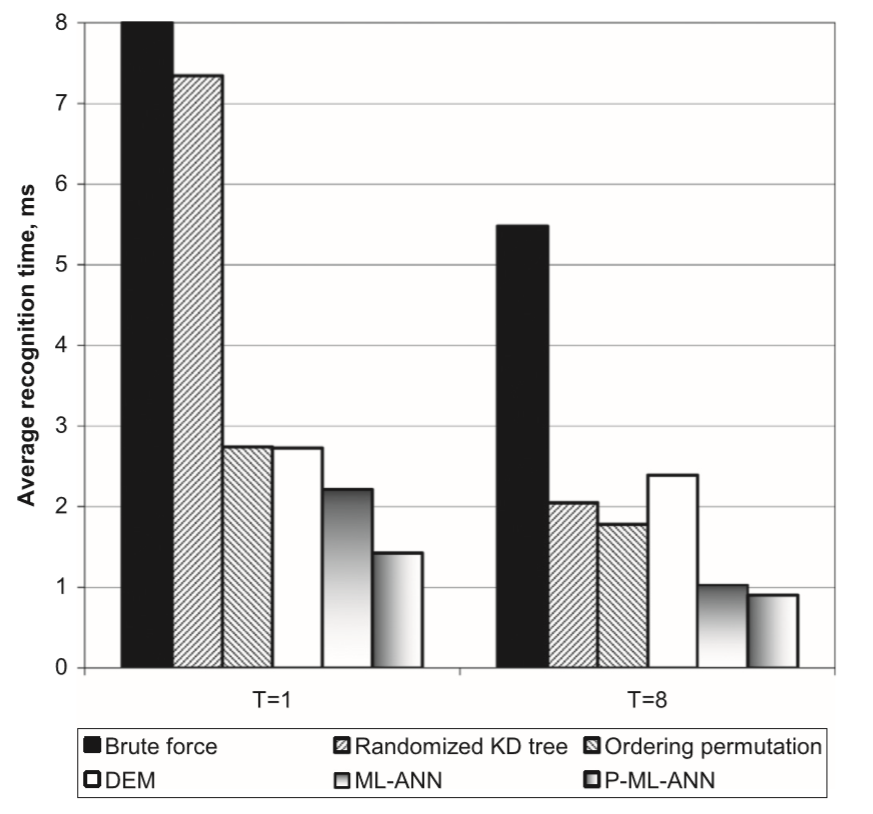
\includegraphics[width=0.7\textwidth]{timings.PNG}
	\caption{Average face recognition time (ms), Euclidean distance, DNN features, LFW dataset.}
	\label{pl1}
\end{figure}

\section{Implementation Dependencies}
\subsection{Anaconda}
This project has been tested with Python 3.6 which is provided in the Anaconda Python package. Anaconda can be downloaded and installed from the official site.

\subsection{Tensorflow}
For this project, we've used the amazing \textit{Tensorflow} framework. The place of usage is illustrated in figure 3.1. To run the project you need the latest version of the \textit{Tensorflow} which can be downloaded using Python package manager, \textit{PIP} using \textit{pip install tensorflow}.

\subsection{OpenCV-Python}
For real-time image pipelining we have used the Python distribution of the OpenCV package. Python OpenCV can be installed with Python package manager with command: \textit{pip install python-opencv}.

\subsection{Pre-trained Model Dependency; Inception Resnet V1}
This model has been trained on the \textit{ImageNet} dataset for feature extraction only. The pre-trained model should be downloaded under the directory \textit{/models}. The model is provided with this report. The model has been implemented by the \textit{Tensorflow} community and is available on the official GitHub repository of Tensorflow.

\subsection{MTCNN-Detect Module}
This module has been implemented by the \textit{David Sandberg} as a part of \textit{Facenet} face recognition and is available via \href{https://github.com/davidsandberg/facenet}{this} link for copyright purposes. The implementation is provided in the directory as \textit{MTCNN-DETECT} module.

\subsection{Core Algorithm}
The core algorithm implementation in Python is provided in the class \textit{Nearest Neighbor}. At the time of writing this paper, the whole method has not been implemented completely in Python and is still in progress, but you can refer to the \textit{ann.cpp} under the \textit{Savchenko} directory for \textit{C++} implementation of the MLANN algorithm.

\subsection{How to Run the Project}
\subsubsection{Adding a New Reference Face}
You can simply open a terminal and type \textit{python main.py --mode input}. Make sure to move your face gradually to extract the features of it!

\subsubsection{Real-time Face Recognition}
You can run the face recognition module using the command \textit{python main.py --mode camera}.